\documentclass[11pt]{beamer}
\usepackage{
	xcolor,
	graphicx,
	subcaption,
	bm,
	pifont,
	booktabs,
	multirow
	} 
%\usefonttheme[onlymath]{serif} % mathmode font like in article TeX	
	
\usetheme{Madrid}

\definecolor{emc-darkblue}{RGB}{14, 36, 112}
\definecolor{emc-lightblue}{RGB}{153, 209, 232}
\definecolor{ggray}{RGB}{208, 208, 208}


\setbeamercolor{palette primary}{bg=emc-darkblue, fg=white}
\setbeamercolor{palette secondary}{bg=emc-lightblue, fg=emc-darkblue}
\setbeamercolor{palette tertiary}{bg=emc-darkblue, fg=white}
\setbeamercolor{structure}{fg=emc-darkblue} 
\setbeamercolor{section in toc}{fg=emc-darkblue} 

\title[EBM Meets Causal Inference]{Evidence-Based Medicine Meets Causal Inference}
\subtitle{Presentation @ Econometric Institute Internal Seminar}


\author[Welz and ten Haaf]{Max Welz \textsuperscript{1} \and Kevin ten Haaf \textsuperscript{2}}
\institute[]{\textsuperscript{1} Erasmus University, Dept. of Econometrics \and \textsuperscript{2} Erasmus MC, Dept. of Public Health}

\titlegraphic{
\includegraphics[width=5cm]{eur-logos/emc-logo.jpg}}

\date[July 21, 2020]{July 21, 2020}

\pgfdeclareimage[height=0.5cm]{university-logo}{eur-logos/eur-stamp.png}
\logo{\pgfuseimage{university-logo}}


% Delete this, if you do not want the table of contents to pop up at
% the beginning of each section:
\AtBeginSection[]
  {
     \begin{frame}
     \frametitle{Outline}
     \tableofcontents[currentsection]
     \end{frame}
  }


%%%%%%%%% bugfix for TeXShop:
\makeatletter
\let\@@magyar@captionfix\relax
\makeatother



%%%%%%%% Bibliography
% capitalization of Dutch names (function applicable to bib file)
\DeclareRobustCommand{\VAN}[3]{#3}

% Note: beamer doesn't support external bib files, so we need to create the bib entries manually like this:
\begin{filecontents}{\jobname.bib}
@article{athey2019grf,
    title = {{Generalized Random Forests}},
    author = {Athey, Susan and Tibshirani, Julie and Wager, Stefan},
    journal = {The Annals of Statistics},
    volume = {47},
    number = {2},
    pages = {1148--1178},
    year = {2019}
}

@article{athey2019grf-appl,
    title = {{Estimating Treatment Effects with Causal Forests: An Appli- cation}},
    author = {Athey, Susan and Wager, Stefan},
    journal = {Observational Studies},
    volume = {5},
    pages = {36--51},
    year = {2019}
}


@article{chernozhukov2018generic,
	title = {{Generic Machine Learning Inference on Heterogeneous Treatment Effects in Randomized Experiments. Technical Report 24678, National Bureau of Economic Research, Cambridge, Massachusetts}},
	author = {Chernozhukov, V and Demirer, M and Duflo, E and Fern\'andez-Val, I},
  year = {2018}
}

@article{dekoning2020,
	author = {{\VAN{Koning}{De}{de}} Koning, Harry J. and van der Aalst, Carlijn M. and de Jong, Pim A. and Scholten, Ernst T. and Nackaerts, Kristiaan and Heuvelmans, Marjolein A. and Lammers, Jan-Willem J. and Weenink, Carla and Yousaf-Khan, Uraujh and Horeweg, Nanda and others},
	journal = {New England Journal of Medicine},
	Title = {{Reduced Lung-Cancer Mortality with Volume CT Screening in a Randomized Trial}},
	year = {2020},
	number = {6},
	volume = {382},
	pages = {503--513}
}


@article{sackett1996,
  title={{Evidence-Based Medicine: What it is and What it isn't}},
  author={Sackett, David L and Rosenberg, William MC and Gray, JA Muir and Haynes, R Brian and Richardson, W Scott},
  year={1996},
  journal={The British Medical Journal},
  volume={312},
  number={7023},
  pages={71--72}
}

@book{shaughnessy2000,
  title={{Research Methods in Psychology}},
  author={Shaughnessy, John J and Zechmeister, Eugene B and Zechmeister, Jeanne S},
  year={2000},
  publisher={McGraw-Hill}
}

@article{kent2018,
  title={{Personalized Evidence Based Medicine: Predictive Approaches to Heterogeneous Treatment Effects}},
  author={Kent, David M and Steyerberg, Ewout and van Klaveren, David},
  journal={The British Medical Journal},
  volume={363},
  year={2018},
  publisher={British Medical Journal Publishing Group}
}

@article{kent2020,
  title={{The Predictive Approaches to Treatment Effect Heterogeneity (PATH) Statement: Explanation and Elaboration}},
  author={Kent, David M and van Klaveren, David and Paulus, Jessica K and D'Agostino, Ralph and Goodman, Steve and Hayward, Rodney and Ioannidis, John PA and Patrick-Lake, Bray and Morton, Sally and Pencina, Michael and others},
  journal={Annals of Internal Medicine},
  volume={172},
  number={1},
  pages={W1--W25},
  year={2020},
  publisher={American College of Physicians}
}

@article{wasserman2009,
  title={{High Dimensional Variable Selection}},
  author={Wasserman, Larry and Roeder, Kathryn},
  journal={The Annals of Statistics},
  volume={37},
  number={5A},
  pages={2178--2201},
  year={2009}
}


\end{filecontents}
 
\usepackage{natbib}
\bibliographystyle{apalike}
% make bibliography entries smaller
\renewcommand\bibfont{\scriptsize}
% If you have more than one page of references, you want to tell beamer
% to put the continuation section label from the second slide onwards
\setbeamertemplate{frametitle continuation}[from second]
% Now get rid of all the colours
\setbeamercolor*{bibliography entry title}{fg=black}
\setbeamercolor*{bibliography entry author}{fg=black}
\setbeamercolor*{bibliography entry location}{fg=black}
\setbeamercolor*{bibliography entry note}{fg=black}
% and kill the abominable icon
\setbeamertemplate{bibliography item}{}


%% tikz options:
\usepackage{tikz}
\usetikzlibrary{arrows.meta}
\usepackage{graphicx}

%% independence symbol
\newcommand\independent{\protect\mathpalette{\protect\independenT}{\perp}}
\def\independenT#1#2{\mathrel{\rlap{$#1#2$}\mkern2mu{#1#2}}}
 
%%%% Let's get started %%%%%
\begin{document}

\begin{frame}
  \titlepage
\end{frame}

\begin{frame}{Outline}
  \tableofcontents
\end{frame}

\section{Introduction}

\begin{frame}{Introduction (1/3)}{Some Context}
	\begin{itemize}
		\item Joint work with the Department of Public Health at Erasmus.
		\item Interdisciplinary project between statistics/econometrics and medicine.
		\item  Initiated as my Master's thesis in econometrics in which I used state-of-the-art causal inferential methods to identify causal heterogeneity in Erasmus MC's NELSON trial
		\begin{itemize}
			\item[$\circ$] NELSON \citep{dekoning2020} is the world's second largest lung cancer screening trial. 
			\item[$\circ$] My thesis' results suggest that standard medical methods for the analysis of RCTs may only capture heterogeneity insufficiently.
		\end{itemize}
		\item[\ding{212}] Show clinicians the added value of incorporating the results of modern causal inferential models in their decision-making.
		\end{itemize}
\end{frame}


\begin{frame}{Introduction (2/3)}{Terminology}
	\begin{itemize}
		\item \alert{Evidence-based medicine}: the ``conscientious, explicit and judicious use of current best evidence in making decisions about the care of individual patients'' \citep{sackett1996}.
		\begin{itemize}
		\item[\ding{212}] Reliable methods to quantify evidence from medical trials are required, especially if there is heterogeneity across subgroups in the trials: Discern signal from noise! 
		\end{itemize}
		\item \alert{Causal inference}: the ``Identification of the cause or causes of a phenomenon, by establishing covariation of cause and effect, a time-order relationship with the cause preceding the effect, and the elimination of plausible alternative causes'' \citep{shaughnessy2000}.
		\item The term \alert{treatment} refers to an economic treatment (which is not necessarily medical) here. 
	\end{itemize}
\end{frame}




\begin{frame}{Introduction (3/3)}{Brief Summary of the Project}
	\begin{itemize}
	\item Medical models for trial evaluations are quite different to the models from causal inference that econometricians are used to.
	\item We demonstrate how modern models from causal inference can yield valuable additional insights for evidence-based and personalized medicine.
	\item We propose to consider the results of an array of medical and causal inferential methods before making medical decisions. 
	\item Target audience: clinicians. We want to raise awareness of the importance of using ``good'' models and therefore aim at a general medical journal.
	\item Relevance: for instance design of future national lung cancer screening programs in order to minimize costs and maximize efficacy (only treat groups that benefit sufficiently).
	\end{itemize}
\end{frame}


\section{Methodology}


\begin{frame}{General Setup: The Potential Outcomes Framework}
	\begin{itemize}
		\item Suppose there are $n$ independent samples $( Y_i, \mathbf{X}_i, W_i)$, indexed by $i$. 
		\begin{itemize}
		\item[$\circ$] The outcome of interest is denoted $Y_i$, the covariates are captured in $p$-vector $\mathbf{X}_i$, and $W_i$ is a binary treatment indicator where $W_i=1$ indicates an assignment to the treatment group and $W_i=0$ to the control group.
		\end{itemize}
	\item Given a realization $\mathbf{X}_i = \mathbf{x}$, the DGP can generally be viewed as
	\[ 
		Y_i(W_i) = \theta(\mathbf{x}) W_i + \nu(\mathbf{x}) + \varepsilon_i,
	\]
	where
	\begin{itemize}
		\item[$\circ$] $\theta(\mathbf{x})$ is the \alert{causal parameter}: the causal effect of $W_i$ on $Y_i$ given $\mathbf{x}$.
		\item[$\circ$] $\nu(\mathbf{x})$ is the \alert{nuisance parameter} which captures the raw effect of $\mathbf{x}$ on $Y_i$ (excluding the effect of treatment $W_i$ on $Y_i$). Usually highly nonlinear!
		\item[$\circ$] $\varepsilon_i$ is an independent noise term that follows some zero-mean distribution.
	\end{itemize}
	\item In practice, we only ever observe one of the two potential outcomes: 
	$Y_i = 
	\begin{cases}
	 Y_i(1) \quad \text{if } W_i=1,\\
	 Y_i(0) \quad \text{if } W_i=0. 
	 \end{cases}$
	 $\implies$ \alert{The fundamental problem!}
	\end{itemize}
\end{frame}


\begin{frame}{Functions of the Causal Parameter}
\[
Y_i = 
\begin{cases}
	 Y_i(1) \quad \text{if } W_i=1,\\
	 Y_i(0) \quad \text{if } W_i=0, 
	 \end{cases}
	 \text{ where }
Y_i(W_i) = \theta(\mathbf{X}_i) W_i + \nu(\mathbf{X}_i) + \varepsilon_i.
\]
\begin{itemize}
	\item An important quantity is the \alert{average treatment effect} (ATE): $\text{ATE} = n^{-1} \sum_{i=1}^n \theta(\mathbf{X}_i)$.
	\begin{itemize}
	\item[$\circ$] If we are in an RCT (that is, random assignment of treatment $W_i$), an unbiased estimate of the ATE is given by 
	$\mathbb{E}[Y_i | W_i=1 ] - \mathbb{E}[Y_i | W_i=0]$.
	\item[$\circ$] RCTs are standard in medicine, so obtaining the ATE is not a problem.
	\end{itemize}
	\item Usually we are interested in estimating group-level ATEs or determining whether there is heterogeneity in $\theta(\mathbf{X}_i)$ and if yes, by what covariates that heterogeneity is driven by: \alert{subgroup analysis}.
	\begin{itemize}
		\item[$\circ$] This is where models from econometrics and medicine start to differ considerably!
	\end{itemize}
\end{itemize}
\end{frame}


\begin{frame}{Subgroup Analysis in Econometrics}
In econometrics, we usually estimate the group-level ATE as a function of per-individual estimates of the causal parameter. For instance,
\begin{itemize}
	\item \cite{chernozhukov2018generic} propose a method for quantifying causal group-level heterogeneity in RCTs that does not rely on strong assumptions.
	\item \cite{athey2019grf} use a random-forest-based GMM-type estimator that yields asymptotically consistent estimates of the causal parameter. A ``doubly-robust'' estimator of group-level ATEs can then be applied on the individual-level estimates of the causal parameter \citep{athey2019grf-appl}. 
\end{itemize}
\alert{Common characteristics of modern econometric causal inference}: \\ 1. Nonparametric (no assumptions on the  shape of the DGP). \\ 2. Able to yield a direct estimate of the group-level ATE. \\
3. Sometimes even an asymptotic theory.
\end{frame}


\begin{frame}{Subgroup Analysis in Medicine (1/14)}{Overview}
\cite{kent2018} distinguish between three types of subgroup analyses in medicine:

\begin{enumerate}
\item One-variable-at-a-time;
\item Risk modeling;
\item Effect modeling.
\end{enumerate}

Each of these methods assumes that outcome $Y_i$ is a binary outcome indicator, that is:
\[
Y_i =
\begin{cases}
1 \quad \text{if individual $i$ gets the outcome within the observation period},\\
0 \quad \text{otherwise}.
\end{cases}
\]
We therefore henceforth assume without loss of generality that $Y_i$ is  a binary mortality indicator.
\end{frame}


\begin{frame}{Subgroup Analysis in Medicine (2/14)}{Type 1: One-variable-at-a-time}
Procedure:
\begin{enumerate}
	\item Partition the samples in subgroups based on their realization of some scalar covariate $X_i$ which is contained in $\mathbf{X}_i$.
	\item Then, given a subgroup, calculate
	\[ 
		Rate Ratio = \frac{(\# \text{Deaths for } W_i=1) / (\# \text{Person-years for } W_i=1)}{(\# \text{Deaths for } W_i=0) / (\# \text{Person-years for } W_i=0)}.
	\]
	(The number of person-years is the sum of the number of years each individual spent in the observation period.) 
	\item Since this is essentially a Poisson counting process, use a Poisson distribution to calculate confidence intervals of the rate ratio.
\end{enumerate}
\end{frame}


\begin{frame}{Subgroup Analysis in Medicine (3/14)}{Type 1: One-variable-at-a-time}
\begin{itemize}
\item Obviously, one-variable-at-a-time analyses are problematic from a causal inference point of view, but they are the \alert{the most often used way of reporting subgroup analyses in medicine.}
\item Some issues: risks for false-negative and false-positive results due to low power for statistical interactions, weak prior theory on potential effect modifiers, and multiplicity. For example, a lower mortality in a subgroup could be caused by the effect of a different variable.
\item[\ding{212}] Can lead to \textit{very} wrong policy recommendations (and already have\dots).
\item The medical literature acknowledges that better methods are needed (\citealp{kent2018}; \citealp{kent2020}).
\end{itemize}
\end{frame}

\begin{frame}{Subgroup Analysis in Medicine (4/14)}{Overview of Predictive Modeling Approaches}
\begin{itemize}
	\item Motivated by the limitations of one-variable-at-a-time analyses, the medical literature suggests to apply predictive modeling for the task of subgroup analysis instead.
	\item It suggests to fit two separate models (recall that $Y_i$ is binary):
	\begin{itemize}
		\item[$\circ$] One to estimate baseline risk $\mathbb{P}(Y_i=1\ |\  \mathbf{X}_i = \mathbf{x}_i)$;
		\item[$\circ$] One to estimate post-treatment risk $\mathbb{P}(Y_i=1\ |\ \mathbf{X}_i = \mathbf{x}_i, W_i = w_i)$.
	\end{itemize}	
	\item This is done to assess by how much the treatment intervention changes the mortality risk.
	\item Two main performance measures:
	\begin{itemize}
		\item[$\circ$] \alert{Calibration}: Ability to match the estimated level of risk closely to the observed level of risk, across different risk-levels;
		\item[$\circ$] \alert{Discrimination}: Ability of the model to distinguish between those with the outcome ($Y_i=1$) and those without the outcome ($Y_i = 0$).
	\end{itemize}
	\item Two main approaches: risk modeling and effect modeling.
	\end{itemize}
\end{frame}


\begin{frame}{Subgroup Analysis in Medicine (5/14)}{Type 2: Risk Modeling}
In risk modeling, we fit the two models, but use the estimated coefficients of the first model to fit the second.
\begin{enumerate}
\item Stage 1: Estimate $(p+1)$ coefficient vector $\bm{\beta}$ in the linear model 
\[
	\mathbb{P}(Y_i=1\ |\  \mathbf{X}_i = \mathbf{x}_i)
	=
	g \Big(\bm{\beta}^\top \mathbf{x}_i^* \Big),
\]
where $\mathbf{x}_i^* = (1, \mathbf{x}_i^\top)^\top$ and $g:\mathbb{R}\to (0,1)$ the logistic function.
\item With $\bm{\hat{\beta}}$, define the linear predictor $\hat{lp}_i = \bm{\hat{\beta}}^\top \mathbf{x}_i^*$.
\end{enumerate}
\end{frame}


\begin{frame}{Subgroup Analysis in Medicine (6/14)}{Type 2: Risk Modeling}
\begin{enumerate}
\setcounter{enumi}{2}
\item Stage 2: Estimate $\bm{\gamma} = (\gamma_0, \gamma_1, \gamma_2)^\top$ in a \alert{separate} linear model
\[
	\mathbb{P}\Big(Y_i=1\ \Big|\ \mathbf{X}_i = \mathbf{x}_i, W_i = w_i, \hat{lp}_i\Big)
	=
	g\Big(
	\hat{lp}_i + \gamma_0 + \gamma_1 w_i + \gamma_2 (w_i \cdot \hat{lp}_i)
	\Big).
\]
\item With $\bm{\hat{\gamma}}$, define post-treatment risk $\hat{\mathbb{P}}_i = g\Big(
	\hat{lp}_i + \hat{\gamma}_0 + \hat{\gamma}_1 w_i + \hat{\gamma}_2 (w_i \cdot \hat{lp}_i)
	\Big)$.
	\item Define the reversed treatment assignment $W_i^{rev}$ by
\[
	W_i^{rev} = 
	\begin{cases}
	1 \quad \text{if } W_i = 0,\\
	0 \quad \text{if } W_i = 1.
	\end{cases}
\]
\end{enumerate}
\end{frame}


\begin{frame}{Subgroup Analysis in Medicine (7/14)}{Type 2: Risk Modeling}
\begin{enumerate}
\setcounter{enumi}{5}
\item Use $W_i^{rev}$ to calculate $
\hat{\mathbb{P}}_i^{rev} = g\Big(
	\hat{lp}_i + \hat{\gamma}_0 + \hat{\gamma}_1 w_i^{rev} + \hat{\gamma}_2 (w_i^{rev} \cdot \hat{lp}_i)
	\Big)$, given $W_i^{rev} = w_i^{rev}$.
\item Calculate absolute and relative predicted benefits $\widehat{apb}_i$ and $\widehat{rpb}_i$, respectively, by 
\begin{align*}
	\widehat{apb}_i &= 
	\begin{cases}
	\hat{\mathbb{P}}_i^{rev} - \hat{\mathbb{P}}_i \quad \text{if } W_i = 1, \\
	\hat{\mathbb{P}}_i - \hat{\mathbb{P}}_i^{rev} \quad \text{if } W_i = 0,
	\end{cases}
	\\
	\widehat{rpb}_i &= 
	\begin{cases}
	\hat{\mathbb{P}}_i / \hat{\mathbb{P}}_i^{rev} \quad \ \ \text{if } W_i = 1,\\
	\hat{\mathbb{P}}_i^{rev} / \hat{\mathbb{P}}_i \quad \ \ \text{if } W_i = 0.
	\end{cases}	
\end{align*}
\item[\ding{212}] $\hat{\mathbb{P}}_i^{rev}$ intends to estimate the counterfactual post-treatment risk.
\end{enumerate}
\end{frame}


\begin{frame}{Subgroup Analysis in Medicine (8/14)}{Type 3: Effect Modeling}
Effect modeling is closely related to risk modeling with the difference that the two fitted models are completely independent of each other.

\begin{enumerate}
\item Baseline risk: Estimate $(p+1)$ coefficient vector $\bm{\beta}$ in the linear model 
\[
	\mathbb{P}(Y_i=1\ |\  \mathbf{X}_i = \mathbf{x}_i)
	=
	g \Big(\bm{\beta}^\top \mathbf{x}_i^* \Big),
\]
where $\mathbf{x}_i^* = (1, \mathbf{x}_i^\top)^\top$ and $g:\mathbb{R}\to (0,1)$ the logistic function.
\end{enumerate}
\end{frame}

\begin{frame}{Subgroup Analysis in Medicine (9/14)}{Type 3: Effect Modeling}
\begin{enumerate}
\setcounter{enumi}{1}
\item Specify $\mathcal{S} \subseteq \{1,\dots,p\}$, which is a set of covariates that are suspected to be treatment effect modifiers/moderators.
\item Consider the linear model
\[
	\mathbb{P}\Big(Y_i=1\ \Big|\ \mathbf{X}_i = \mathbf{x}_i, W_i = w_i\Big) 
	=
	 g\Bigg(
	 \bm{\alpha}^\top \mathbf{x}_i^*
	 +
	 \sum_{\{j : j \in \mathcal{S}\}} \delta_j w_i x_{ij}
	 \Bigg)
\]
and gather its coefficients in the ($k+1$) coefficient vector $\bm{\gamma} = (\bm{\alpha}^\top, \{\delta_j \}^\top_{j\in \mathcal{S}} )^\top = (\gamma_0, \gamma_1, \dots, \gamma_k)^\top$, where $k = p + |\mathcal{S}|$. 
The $\delta_j$ are the coefficients of interaction terms $w_ix_{ij}$.
\item Fit $\mathbb{P}(Y_i=1\ |\ \mathbf{X}_i = \mathbf{x}_i, W_i = w_i)$ by means of penalized logistic regression (lasso here) and obtain $\bm{\hat{\gamma}}$.
\end{enumerate}
\end{frame}


\begin{frame}{Subgroup Analysis in Medicine (10/14)}{Type 3: Effect Modeling}
\begin{enumerate}
\setcounter{enumi}{4}
\item Let $\mathcal{U} = \{j: \hat{\gamma}_j \neq 0, j \neq 0\} \subseteq \{1,\dots,k\}$ be the set of variables retained by the lasso, and $\mathcal{R} = \mathcal{U} \setminus \{j: j \in \mathcal{U}, j > p \}$ be the set of the retained variables that are \textit{not} interaction effects.
\item Fit two separate ordinary logistic regression models: 
\begin{itemize}
	\item[$\circ$] An \alert{unrestricted} model of $Y_i$ on variable set $\mathcal{U}$,
	\item[$\circ$] A \alert{restricted} model of $Y_i$ on variable set $\mathcal{R}$.
\end{itemize}
\item Using the restricted and unrestricted model, perform a likelihood ratio test on joint significance of the coefficients of the interaction effects. If we reject joint significance, use the restricted model as final model. Otherwise, use the unrestricted model as final model.
\item Note: We use three separate random non-overlapping sets of samples for the three tasks of estimation, evaluation, and hypothesis testing, as suggested by \cite{wasserman2009}.
\end{enumerate}
\end{frame}

\begin{frame}{Subgroup Analysis in Medicine (11/14)}{Type 3: Effect Modeling}
\begin{enumerate}
\setcounter{enumi}{8}
\item Use the final effect model to obtain predictions of the post-treatment risk, $\hat{\mathbb{P}}_i = \hat{\mathbb{P}}(Y_i=1\ |\ \mathbf{X}_i = \mathbf{x}_i, W_i = w_i)$, of all samples. 
\item Use reversed treatment assignment $W_i^{rev}$ to obtain predictions of the counterfactual risk: $\hat{\mathbb{P}}_i^{rev} = \hat{\mathbb{P}}(Y_i=1\ |\ \mathbf{X}_i = \mathbf{x}_i, W_i = w_i^{rev})$.
\item Analogously to risk modeling, calculate absolute and relative predicted benefits $\widehat{apb}_i$ and $\widehat{rpb}_i$, respectively, by 
\begin{align*}
	\widehat{apb}_i &= 
	\begin{cases}
	\hat{\mathbb{P}}_i^{rev} - \hat{\mathbb{P}}_i \quad \text{if } W_i = 1, \\
	\hat{\mathbb{P}}_i - \hat{\mathbb{P}}_i^{rev} \quad \text{if } W_i = 0,
	\end{cases}
	\\
	\widehat{rpb}_i &= 
	\begin{cases}
	\hat{\mathbb{P}}_i / \hat{\mathbb{P}}_i^{rev} \quad \ \ \text{if } W_i = 1,\\
	\hat{\mathbb{P}}_i^{rev} / \hat{\mathbb{P}}_i \quad \ \ \text{if } W_i = 0.
	\end{cases}	
\end{align*}
\end{enumerate}
\end{frame}


\begin{frame}{Subgroup Analysis in Medicine (12/14)}{Processing the Predicted Benefits}
Suppose we have obtained the quantities of absolute and relative predicted benefits $\widehat{apb}_i$ and $\widehat{rpb}_i$, respectively, from a predictive model. Thereupon, we're interested in evaluating heterogeneity in the treatment effectiveness.
\begin{enumerate}
\item Group the samples into $q$ groups based on the quantiles of the baseline risk $\mathbb{P}(Y_i=1\ |\  \mathbf{X}_i = \mathbf{x}_i)$, which was estimated in the first modeling stage. Denote by $G_i \in \{ 1,\dots, q\}$ the group membership.
\item For each group $G_i = g$, calculate the \textit{observed benefit} $\widehat{ob}_g$: 
\begin{align*}
	\widehat{ob}_g = 
	&|\{i : G_i=g, W_i=1 \}|^{-1}
	\sum_{\{i : G_i=g, W_i=1 \}} Y_i
	\ -\\
	&|\{i : G_i=g, W_i=0 \}|^{-1}
	\sum_{\{i : G_i=g, W_i=0 \}} Y_i,
\end{align*}
which is essentially an estimate of the group-level ATE.
\end{enumerate}
\end{frame}

\begin{frame}{Subgroup Analysis in Medicine (13/14)}{Processing the Predicted Benefits}
\begin{enumerate}
\setcounter{enumi}{2}
\item Furthermore, for each group $G_i = g$, calculate the group-level \textit{predicted benefit} by taking the within-group mean. For instance, for the absolute predicted benefits $\widehat{apb}_i$,
\[
	\widehat{apb}_g = |\{ i: G_i = g \}|^{-1} \sum_{\{i: G_i = g\}} \widehat{apb}_i.
\]
\item[\ding{212}] Intends to average out the noise of the noisy individual estimates $\widehat{apb}_i$.
\end{enumerate}
Recall now that a model is considered to be ``good'' if it is calibrated well, that is, if $\widehat{ob}_g \approx \widehat{apb}_g$ for all $g=1,\dots,q$. Assess by \alert{calibration plots} in which the $\widehat{ob}_g$ and $\widehat{apb}_g$ are plotted against each other.
\end{frame}


\begin{frame}{Subgroup Analysis in Medicine (14/14)}{Comments on the Predictive Models}
\begin{itemize}
\item Aside from the two general assumptions of unconfoundedness ($ (Y_i(0), Y_i(1))\independent W_i \big| \mathbf{X}_i$) and sufficient overlap ($\mathbb{P}(W_i = 1 | \mathbf{X}_i = \mathbf{x}) \in (0,1)$), the two types of predictive models rely on the linearity assumption on the DGP.
\item[\ding{212}] Might be too restrictive for valid causal inference.
\item The requirement \textit{observed benefit} $\approx$ \textit{predicted benefit} relies on meaningful grouping based on baseline risk $\mathbb{P}(Y_i = 1 | \mathbf{X}_i = \mathbf{x})$. But this is unknown and estimating it with linear models might fail to capture heterogeneity.
\item No underlying statistical theory. However, they resemble to some extent \textit{generic machine learning} \citep{chernozhukov2018generic}, so maybe it is possible to derive one\dots.
\end{itemize}
\end{frame}


\section{Simulation}


\begin{frame}{A Simple Data Generating Process}
In order to demonstrate how predictive models work, we apply them on $n=10,000$ i.i.d. samples generated by the following simple process.
\begin{itemize}
\item $\mathbf{X}_i \sim \mathcal{N}_5 \big(\mathbf{0}, \mathbf{I} \big), \varepsilon_i \sim \mathcal{N}(0, 0.5^2), \bm{\beta} = (0.2, 0.5, -0.3, 0.7, -0.1, 0.4)^\top$;
\item Set $z_i = (1, \mathbf{x}_i^\top) \cdot \bm{\beta} + \varepsilon_i$ for $\mathbf{X}_i = \mathbf{x}_i$;
\item Calculate $\pi_i(0) = \mathbb{P}(Y_i=1 | \mathbf{X_i}=\mathbf{x}_i, W_i=0)= \text{logistic}(z_i)$; 
\item Set $\pi_i(1) = \mathbb{P}(Y_i=1 | \mathbf{X_i}=\mathbf{x}_i, W_i=1) = 0.7 \cdot \pi_i(0)$ to model a \alert{constant relative treatment effect} across all treated individuals;
\item Draw $Y_i(W_i) \sim \text{Bernoulli}(\pi_i(W_i))$ for $W_i = 0,1$; 
\item Draw $W_i \sim \text{Bernoulli}(0.5)$ and determine the observed outcome 
$Y_i =
\begin{cases}
Y_i(1) \quad \text{if } W_i=1, \\
Y_i(0) \quad \text{if } W_i=0.
\end{cases}
$
\item[\ding{212}] $Y_i$ is a binary mortality indicator and treatment $W_i$ reduces the relative mortality risk by 30\%.
\item[\ding{212}] $ATE = n^{-1} \sum_{i=1}^n \big( \pi_i(1) - \pi_i(0) \big) \approx -0.162$.
\end{itemize}
\end{frame}


\begin{frame}{Performance of the Predictive Models}
Performance on a representative generated dataset. Note that the models produce positive estimates for the predicted benefits to facilitate interpretation. Further recall $ATE\approx -0.162$ and $W_i$ induces a relative mortality reduction of 30\%.\\
\medskip
The risk model:
\begin{itemize}
	\item $n^{-1}\sum_{i=1}^n \widehat{apb}_i = 0.164$,
	\item $1-n^{-1}\sum_{i=1}^n \widehat{rpb}_i = 0.32$. 
\end{itemize}
The effect model:
\begin{itemize}
	\item $n^{-1}\sum_{i=1}^n \widehat{apb}_i = 0.162$,
	\item $1-n^{-1}\sum_{i=1}^n \widehat{rpb}_i = 0.325$. 
\end{itemize}
The estimated coefficients of both models furthermore correctly suggest that there are no interaction effects.
\end{frame}


\begin{frame}{Calibration Plots of the Risk Model}
\begin{figure}
\centering
	\begin{subfigure}{0.49\textwidth}
		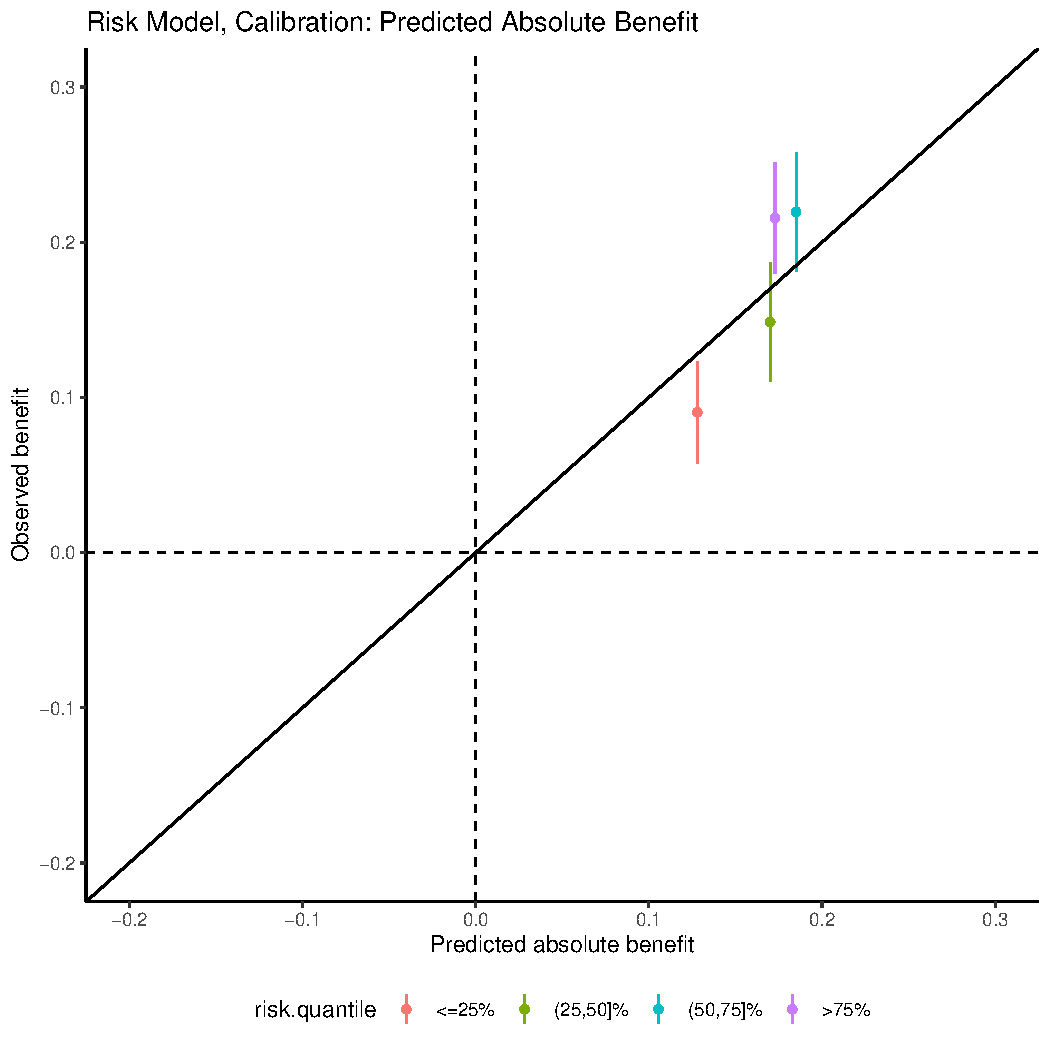
\includegraphics[width=\linewidth]{plots/const-rm-calibration-absolute.pdf}
		\caption{Group-level absolute benefit}
	\end{subfigure}
	\begin{subfigure}{0.49\textwidth}
		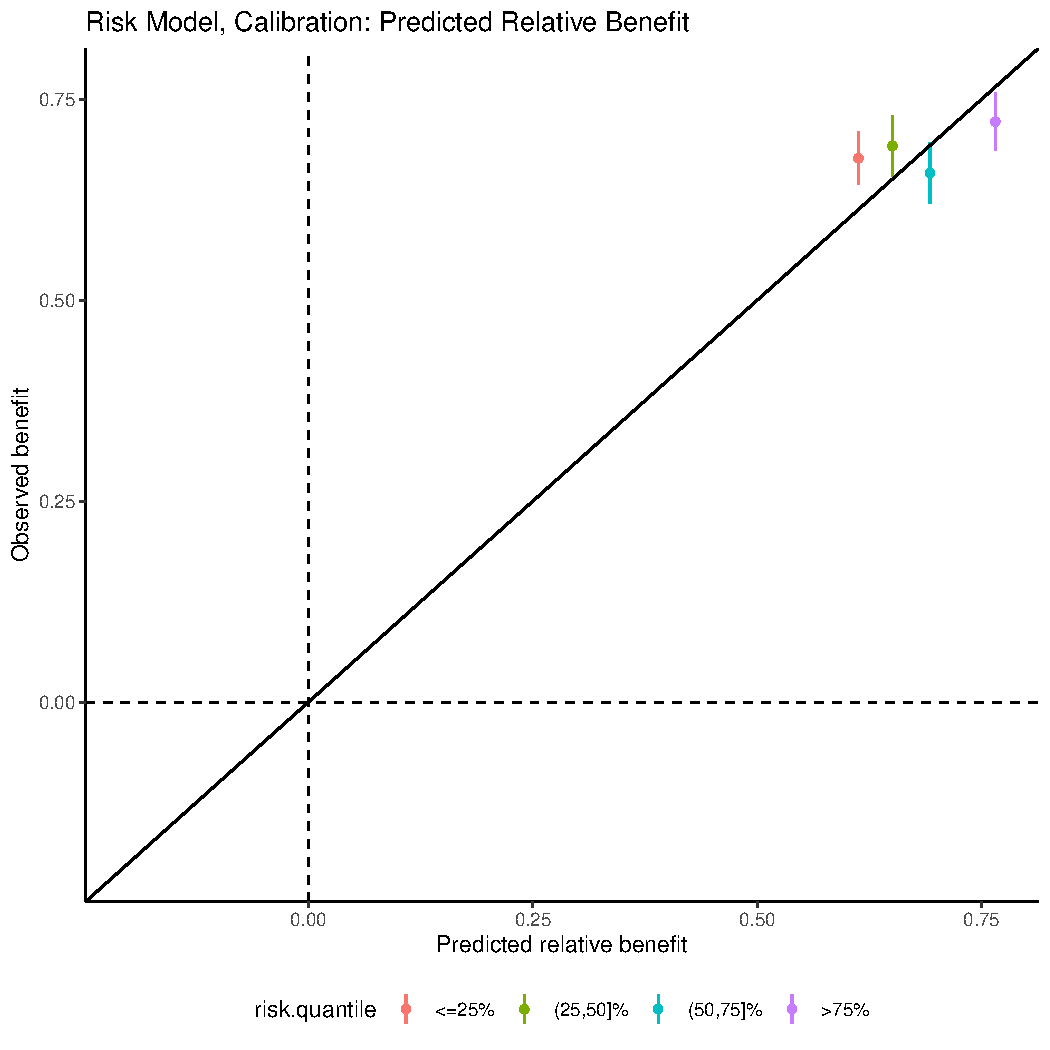
\includegraphics[width=\linewidth]{plots/const-rm-calibration-relative.pdf}
		\caption{Group-level relative benefit}
	\end{subfigure}
\medskip \\

Left panel: group means are close to the $45^\circ$ line \ding{212} Good calibration. 		
Right panel: Constant relative benefits \ding{212} No heterogeneity.
\end{figure}
\end{frame}

\begin{frame}{Calibration Plots of the Causal Forest}
\begin{itemize}
\item A ``causal'' random forest \citep{athey2019grf} estimates the causal parameter of interest $\theta(\mathbf{x}_i)$, given $\mathbf{X}_i = \mathbf{x}_i$, for each individual $i=1,\dots,n$. This is a nonparametric method!
\item Since $Y_i$ is binary, $\theta(\mathbf{x}_i)$ is interpreted as treatment-induced reduction in mortality risk.
\item[\ding{212}] This corresponds to the absolute predicted benefit!
\item Unfortunately, the causal forest does not allow for the estimation of the relative predicted benefit.
\item[\ding{212}] Evaluate heterogeneity by, for instance, plotting $\hat{\theta}(\mathbf{x}_i)$ against each covariate.
\item Estimate baseline risk through ordinary regression forest of $Y_i$ on $\mathbf{X}_i$ (nonparametric again).
\end{itemize}
\end{frame}

\begin{frame}{Calibration Plot of the Causal Forest}
\begin{figure}
\centering
		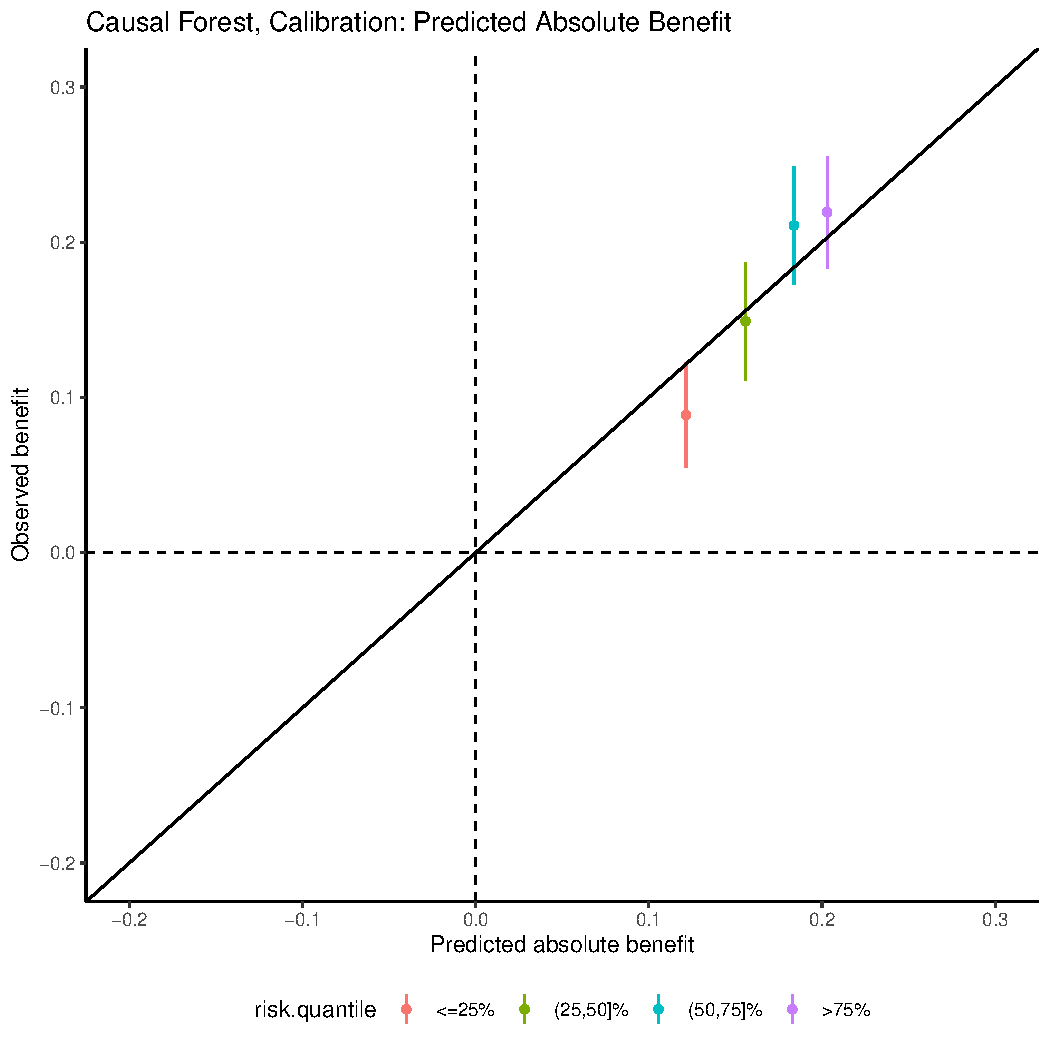
\includegraphics[width=0.5\linewidth]{plots/const-cf-calibration-absolute.pdf}
\end{figure}
Good calibration! Also, accurate estimation of ATE: estimated to be $-0.166$ and plotting the $\hat{\theta}(\mathbf{x}_i)$ against each covariate correctly does not indicate heterogeneity.
\end{frame}


\begin{frame}{Calibration Plot of Generic Machine Learning}
Working generic machine learning \citep{chernozhukov2018generic} into this framework is still work in progress! Same goes for survival models.
\end{frame}

\section{Conclusion}

\begin{frame}{Conclusion}
To-Do-List:
\begin{itemize}
	\item Conceive a large-scale simulation with a nonlinear DGP. Preliminary results suggest that the predictive models break down, whereas the modern causal inferential methods do not.
	\item Investigate how the modern methods perform in relatively small sample sizes.
	\item Finalize an \textsf{R} package which provides flexible and user-friendly functions for the estimation and analysis of predictive models in medicine.
	\item Apply the predictive models on the data of the NELSON trial.
\end{itemize}
\alert{Main point}: We want to demonstrate to clinicians that they should consider several different models before they engage in medical decision making (evidence-based medicine!). By doing so, they get a better understanding of the factors driving treatment effect heterogeneity and therefore become more certain that recommending an alternative treatment for a group might be the ``right thing'' to do.
\end{frame}


\begin{frame}
\centering \Huge{Thanks for you attention! Any questions?}
\end{frame}







\begin{frame}[t,allowframebreaks]
\frametitle{References}
\bibliography{\jobname}
\end{frame}

% TODO: include causal graph? Mention that early stage detection means better prognosis. Mention imputation
\end{document}